\documentclass{article}

\renewcommand{\familydefault}{\sfdefault}  %serifenlose Schrift
\usepackage{helvet} % Schrift: Helvetica


\usepackage{graphicx,graphics,tikz}
\usepackage{amsmath}
\usepackage{amsthm}
\usepackage{amsfonts}
\usepackage{amssymb}
\usepackage{marvosym} % to be able to show male and female symbols with: \Female and \Male
\usepackage{gensymb}
\usepackage[graphics,tightpage,active]{preview}
\PreviewEnvironment{tikzpicture}
\newlength\imagewidth
\newlength\imagescale

\begin{document}

\pgfmathsetlength{\imagewidth}{10cm} % desired displayed width of image
\pgfmathsetlength{\imagescale}{\imagewidth/2000} % pixel width of image
% adjust scale of tikzpicture (and direction of y) such that pixel
% coordinates can be used for drawing overlays:
\usetikzlibrary{backgrounds}

\begin{tikzpicture}[scale=0.8,font=\sffamily]
\draw [line width=0.1cm,-latex] (0,0) -- (10,0);
\draw [line width=0.1cm,-latex] (0,0) -- (0,5);

\node [scale=1] at (0,5.3) {\textbf{Fitness}};
\node [scale=1] at (11.4,0) {\textbf{Temperature}};

\draw [line width=0.08cm] plot[domain=1.5:8,smooth] (\x,-{sin(\x r)}+1);

% Orange photosynthetic performance
\draw [color=orange,line width=0.05cm] plot[domain=1.5:8,smooth] (\x,-{sin(\x r)}*0.5+0.5);

% Delimitation of stress

%\draw [dashed,gray] (3.5,0)--(3.5,3);
%\draw [dashed,gray](6,0)--(6,3);

\shade[left color=white,right color=black] (4.75,-0.5) rectangle (7.75,-0.1);
\shade[right color=white,left color=black] (4.75,-0.5) rectangle (1.75,-0.1);

\node [scale=0.8] at (4.75,-0.8){Benign};
\node [scale=.8] at (3,-0.8){Stress};
\node [scale=.8] at (6.5,-0.8){Stress};
\node [scale=.8] at (1.75,-0.8){Lethal};
\node [scale=.8] at (7.75,-0.8){Lethal};

\draw [-latex,color=orange,line width=0.05cm] (1.5,0) -- (1.5,3);
\node  [color=orange,rotate=90,scale=.8,text width=3cm,text centered] at (1,1.6) {Photosynthetic performance};

\node [color=orange,anchor=west] at (2cm,4cm){Fluorescence measurements};

\draw [color=orange,line width=0.05cm] (6,-1.2) -- (7.8,-1.2);
\node[anchor=north west,inner sep=0pt,outer sep=0pt,scale=1] at (8cm,4cm) {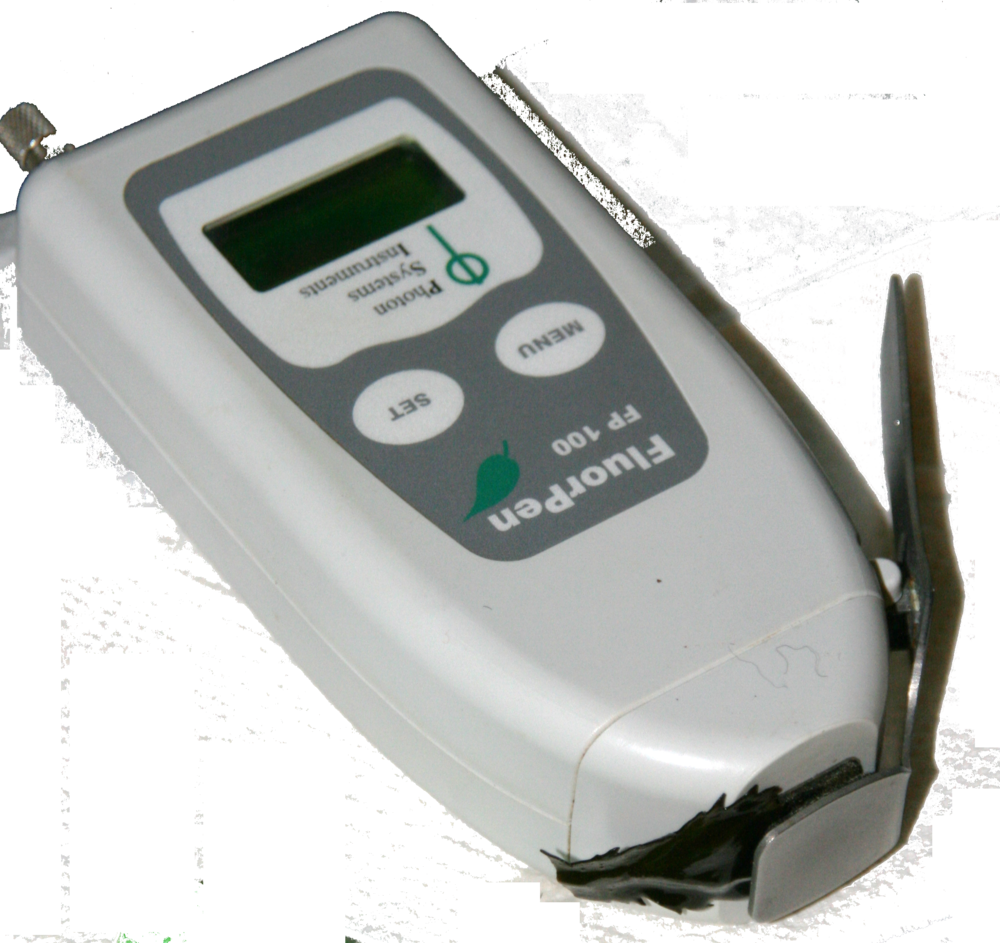
\includegraphics[width=2cm]{Fluorometer_r.png}};
\node [color=orange,scale=.8] at (6.9,-1.5) {20\celsius--28\celsius};

\end{tikzpicture}

\end{document}